%%%%%%%%%%%%%%%%%%%%%%%%%%%%%%%%%%%%%%%%%%%%%%%%%%%%%%%%%%%%%%%%%%%%%%%%%%%%%%%%%%%%%%%%%%%%%%%
\begin{figure}[t!]
    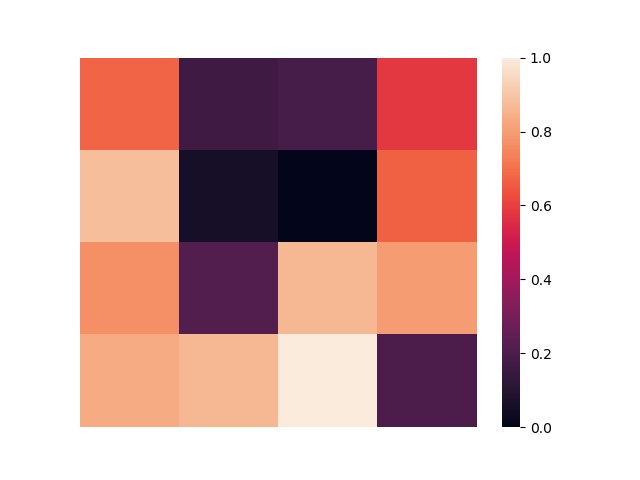
\includegraphics[width=\linewidth]{data/max_heatmap.png} 
    \caption{Heat map that shows the max reward provided from the reward model to the policy. That is computed after the reward model early stop.}
	\label{fig:heatmap}%
\end{figure}
%%%%%%%%%%%%%%%%%%%%%%%%%%%%%%%%%%%%%%%%%%%%%%%%%%%%%%%%%%%%%%%%%%%%%%%%%%%%%%%%%%%%%%%%%%%%%%%

\section{Conclusions}
The aim of this project is to verify the effectiveness of the proposed method by \textit{Borja Ibarz et all.}\ \cite{NIPS2018_8025}, without the human demonstrations. The aim of our project is to force the agent to learn a sub optimal trajectory in the Minigrid environment. This is achieved using the Inverse Reinforcement Learning method: the agent does not take the reward from the environment but there is a reward model that predicts this from agent observations. 

So we define an architecture able to train the agent following our "forced trajectory". Thanks to this, the reward model learns to give high reward to the agent when he is in the forced trajectory states and small reward when the agent is in other states.

The experiments have been carried out in the Minigrid empty environment 6x6, but we believe that this system will work with all the other environment. In particular, the more complex the environments will be, the greater the benefits of the usage of an IRL system will be. This is because in complex environment, the agent will reach the goal state easily using rewards given by a reward model, instead of by the environment. This will reduce the training time, because the agent will not do initial random actions, but he will mimics the human expert behaviour. 
So the user can control step by step what the agent learns from the environment, expressing what the agent has to do in the environment.